\documentclass[12pt,a4paper]{article}
\usepackage{amsmath,amssymb,amsthm,epsf, graphicx, rotating}
\usepackage{fancyhdr}
\usepackage{subfig}
\usepackage{float}
\graphicspath{ {./images/} }

\pagestyle{empty}
\setlength{\parindent}{0pt}
\setlength{\textwidth}{6.5in}
\setlength{\oddsidemargin}{0in}
\addtolength{\textheight}{1in}

\renewcommand\theenumi{\alph{enumi}}
\renewcommand\labelenumi{(\theenumi)}

\newcommand{\Z}{\mathbb{Z}}
\newcommand{\F}{\mathbb{F}}
\newcommand{\R}{\mathbb{R}}
\newcommand{\C}{\mathbb{C}}
\newcommand{\N}{\mathbb{N}}
\renewcommand\vec{\mathbf}

\pagestyle{fancy}
\fancyhf{}
\fancyhead[LE, RO]{Ryan Liu}

\theoremstyle{definition}
\newtheorem{problem}{}

\author{Ryan Liu}
\title{MATH 442 Homework 5}
\begin{document}

\begin{center}
{\huge MATH 442 \par}
{\Large Homework  5  \par}
{\normalsize Name: Ryan Zhuo Lun Liu \par}
{\normalsize Student Number: 30328141 \par}
{\normalsize Collaborators: Jagjot Jhajj and Robert Benjamin Lang }
\end{center}

\begin{problem} \underline{Answer:} This will be proved using Induction. \\
\underline{Base Case:} \\
The tree with two vertices is $T(2)$, which has one edge and two vertices of degree one. \\

\underline{Induction Step:} \\
Suppose that the statement is true for $n$ vertices, prove that the statement is true $n + 1$ vertices. \\

For any tree, it must be true that it cannot contain a cycle, else it would no longer be a tree. \\

Let $G$ be a tree with $n$ vertices. Since it has $n$ vertices, it follows that it has at least one vertex with degree one. \\

Suppose $G'$ is the tree obtained by adding a vertex $x$ to $G$, we see that there are two cases. We can add $x$ by adding exactly one edge and thus $x$ is of degree one and the statement is true. We can also add the vertex to multiple different vertices in $G$, but that would require adding additional edges and would be an illegal move for trees as it would create a cycle. Thus, in order for for $G'$ to remain a tree, we can only add one extra edge and create another vertex of degree one.

\end{problem}

\begin{problem} \underline{Answer: } \\
If $G$ is a (simple) planar graph with $v$ vertices, $e$ edges and $f$ faces, then it is true that $v - e + f = 2$. \\

Since $G$ contains no cycles of length $\leq$ k, that means that a face must be bounded by a cycle of at least $k + 1$ edge sides. Using the definition of $x$ from class, we have that $x = 2e$ and $x \geq (k + 1)f$. \\

Using the formula above, we see that $f = 2 - v + e$ and using the above formulas, we have $x = 2e \geq (k + 1)f \rightarrow 2e \geq (k + 1)(2 - v + e)$. \\

Simplifying the above expression: \\
$= 2e \geq 2k - kv + ek + 2 - v + e$ \\
$= e \geq 2k - kv + ek + 2 - v$ \\
$= e - ek \geq 2k - kv + 2 - v$ \\
$= ke - e \leq kv - 2k + v - 2$ \\
$= (k - 1)e \leq (k + 1)(v - 2)$ \\
$= e \leq \frac{(k + 1)(v - 2)}{k - 1} \leq \frac{(k + 1)(v)}{k - 1}$ if $v \geq 2$\\

\end{problem}

\begin{problem}

By definition, a closed path is a walk with distinct vertices and edges that starts and ends at the same vertex. Proving by the contrapositive, the statement becomes that if a graph $G$ is not bipartite, then $G$ contains a closed path of odd length. \\

Suppose that $G$ is bipartite, the graph can be separated into two distinct sets (Black and White). Let $x$ be a vertex in the Black set and let $y$ be a vertex in the White set. To construct a closed path, we must start and end at $x$ or $y$ while traversing distinct edges and vertices. \\

As each vertex in the Black set is only connected to vertices in the White set and vice versa, we see that closed paths in $G$ have to be of even length. If there existed a closed path of odd length, then it would mean that two vertices in the Black (or White) set are connected, meaning that $G$ is not bipartite. \\

Thus, if $G$ contained a closed path of odd length, then $G$ is not bipartite. As the contrapositive is true, the original statement must be true as well.

\end{problem}

\begin{problem}

Using Eurler's Theorem, we know that $v - e + f = 2$. In this situation, this planar graph has 9 vertices and $\frac{5*4 + 4*3}{2} = 16$ edges. Thus, it has $f = 2 - v + e \rightarrow 2 - 9 + 16 = 9$ faces.

\begin{figure}[H]
    \centering
    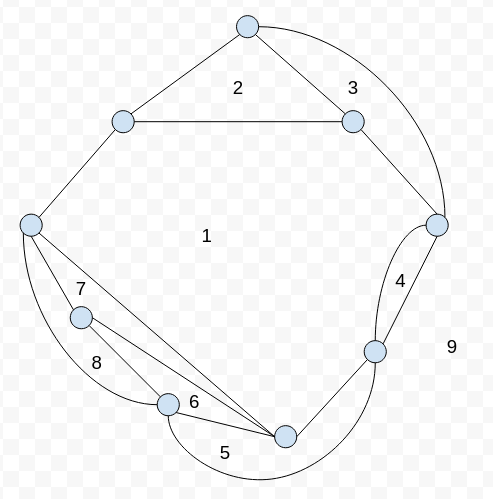
\includegraphics[scale=0.6]{q4.png}
    \caption{Example Graph}
    \label{fig:my_label}
\end{figure}

\end{problem}

\begin{problem}

As proved in homework 3, $Q_k$ has $2^k$ vertices and $k(2^{k-1})$ edges. In addition, $Q_k$ cannot have a cycle of length 3 as it is impossible to have three binary numbers to be one digit away from each other.

As $Q_k$ is a simple connected graph, to be planar, $e \leq 2v - 4$. We proved this in class. \\

Given the above, we see that: we must fulfill $k(2^{k - 1}) \leq 2(2^k) - 4$. \\

The above condition can be simplified to: $k \leq 2^2 - \frac{4}{2^{k - 1}} \rightarrow k \leq 4 - \frac{4}{2^{k - 1}} < 4$\\

Thus, $Q_k$ is planar when $k < 4$.

As the formula only works for graphs with vertices $v > 2$, refer to the figure below for a planar drawing of $Q_1$ and $Q_2$.

\begin{figure}[H]
    \centering
    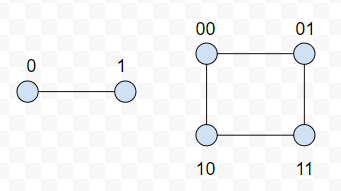
\includegraphics[scale=0.6]{q5.png}
    \caption{$Q_1$ and $Q_2$}
    \label{fig:my_label}
\end{figure}

\end{problem}

\begin{problem}

Suppose that $G$ is a planar graph with $< 12$ vertices that each vertex has degree $\geq 5$. \\

Thus, we have that $S = \sum_{v \in V} d(v) > 5v$. \\

Given that $2e = S$, we have that: $5v \leq S = 2e \leq 6v - 12 \rightarrow v \geq 12$. \\

Thus, the degree of vertices in $G$ must be $\leq 4$.

\end{problem}

\begin{problem}

Suppose graph $G$ is a simple planar graph with $e$ edges and $v$ vertices. Since we have $v \geq 11$, we can say that $e \leq 3v - 6$. \\

$\overline{G}$ would have $v$ vertices but $\frac{v(v - 1)}{2} - e$ edges. Suppose that $\overline{G}$ is also a simple planar graph, then it must also satisfy the same condition above, mainly that: $\frac{v(v - 1)}{2} - e \leq 3v - 6$. \\

Adding the two inequalities together, we get: $\frac{v(v - 1)}{2} \leq 6v - 12 \rightarrow v \leq 10$. \\

Thus, if $G$ is a simple graph with $v \geq 11$, $G$ and $\overline{G}$ cannot both be planar.

\end{problem}

\end{document}
